\chapter{Polígonos y extrusiones}

\section{Polígonos}


\lettrine[ante=\raisebox{-1.5ex}{\Large ---},lines=2]{S}{upongo que}
uniendo y cortanto cubos, cilindros y esferas podrían lograrse todos
los objetos imaginables; he ahí un bonito teorema para demostrar
---conjeturó Antonia---. En cualquier caso, es bueno saber que
\openscad{} nos brinda otras posibilidades: por ejemplo, crear una
superficie bidimensional para luego extenderla perpendicularmente. Una
de esas superficies es el \lstinline!polygon!.

  \begin{figure}[ht]
  \begin{minipage}[]{.5\textwidth}%\vspace{0pt}
    \begin{lstlisting}
polygon([[-20,-20],
         [-10,0],
         [-20,20],
         [20,20],
         [10,0],
         [20,-20]]);
    \end{lstlisting}
  \end{minipage}\hfill
  \begin{minipage}[]{.5\textwidth}%\vspace{0pt}
      \flushright
      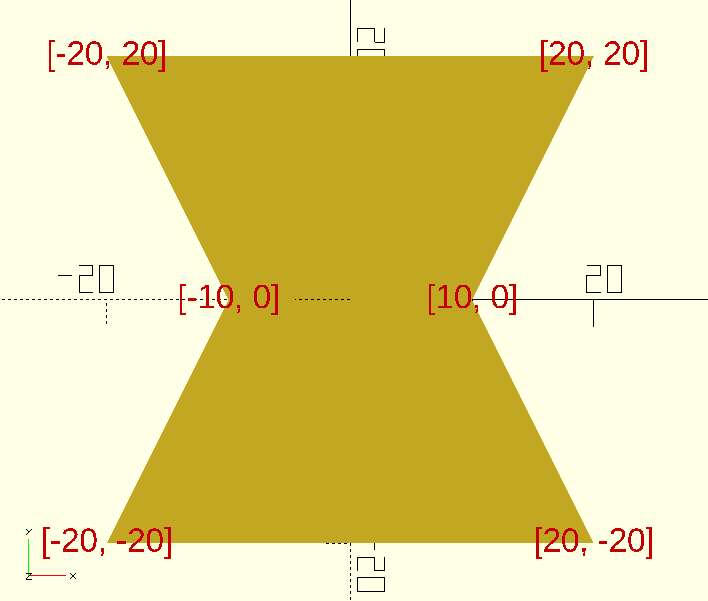
\includegraphics[width=.95\textwidth]{imagenes/poligono-1}
    \end{minipage}
    \caption{Antonia crea un \lstinline!polygon! a manera de ejemplo.}
    \label{fig:poligono-1}
  \end{figure}


  \guillemotright\lstinline!polygon! recibe como parámetro una matriz
  con los puntos que lo definen ---explicó Antonia---. Cada uno de
  ellos representa un punto en el plano \coord{XY}: el primer número
  del punto es la coordenada en \coord{X}, y el otro la posición en
  \coord{Y}; por supuesto, al tratarse de una figura 2D dichos puntos
  no tienen coordenada \coord{Z}.  \openscad{} los une entonces, en
  orden, mediante segmentos. El último punto se une automáticamente
  con el primero: en el caso de la figura \ref{fig:poligono-1}, el
  punto \lstinline![20,-20]! con el \lstinline![-20,-20]!.

  \guillemotright Si vos mirás el polígono de soslayo ---advirtió
  Antonia--- te va a aparecer con un pequeño espesor; pero que
    no te confunda: es una característica del motor gráfico que emplea
    \openscad{} para visualizar los objetos. Los polígonos,
    internamente y de acuerdo con la más elemental geometría, no
    tienen espesor. De paso, te confirmo que los puntos pueden
    aludirse con una variable.

    \vfill
    
  \begin{figure}[ht]
  \begin{minipage}[]{.4\textwidth}%\vspace{0pt}
    \begin{lstlisting}
puntos=[[-20,-20],
        [-10,0],
        [-20,20],
        [20,20],
        [10,0],
        [20,-20]];
         
polygon(puntos);
    \end{lstlisting}
  \end{minipage}\hfill
  \begin{minipage}[]{.6\textwidth}%\vspace{0pt}
      \flushright
      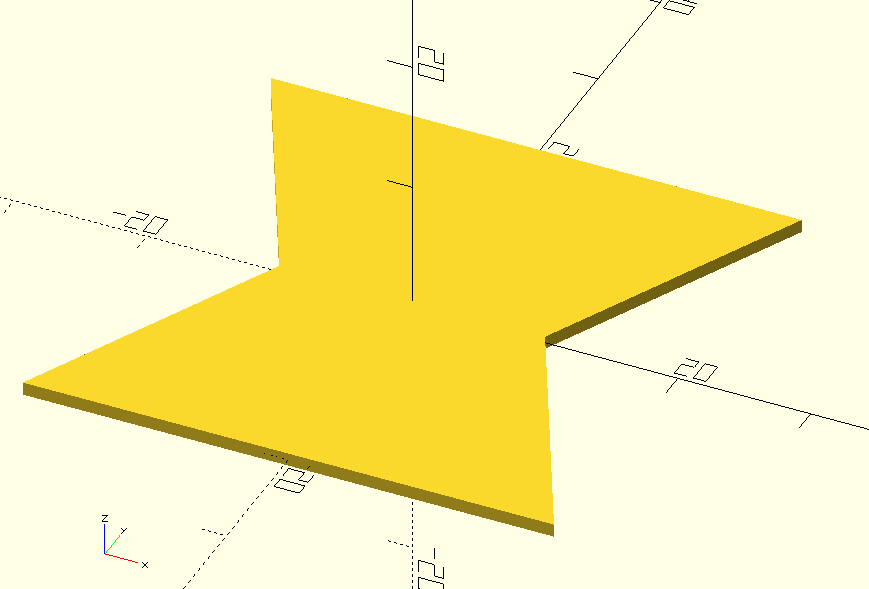
\includegraphics[width=.95\textwidth]{imagenes/poligono-soslayo}
    \end{minipage}
    \caption{\lstinline!polygon! definido a partir de una variable. El
      espesor que se aprecia es un artificio del motor gráfico de
      \openscad{}: internamente y como la más elemental geometría
      impone, es nulo.}
    \label{fig:poligono-soslayo}
  \end{figure}



  \section{Extrusión lineal}

  ---Hay varias operaciones que te permiten erigir un objeto 3D con
  una figura plana; quizá la más elemental sea la ofrecida por
  \lstinline!linear_extrude! ---dijo Antonia, mientras tecleaba con su
  rapidez habitual.

  \begin{figure}[ht]
  \begin{minipage}[]{.5\textwidth}%\vspace{0pt}
    \begin{lstlisting}
puntos=[[-20,-20],
        [-10,0],
        [-20,20],
        [20,20],
        [10,0],
        [20,-20]];

linear_extrude(100)         
  polygon(puntos);
\end{lstlisting}
  \end{minipage}\hfill
  \begin{minipage}[]{.5\textwidth}%\vspace{0pt}
      \centering
      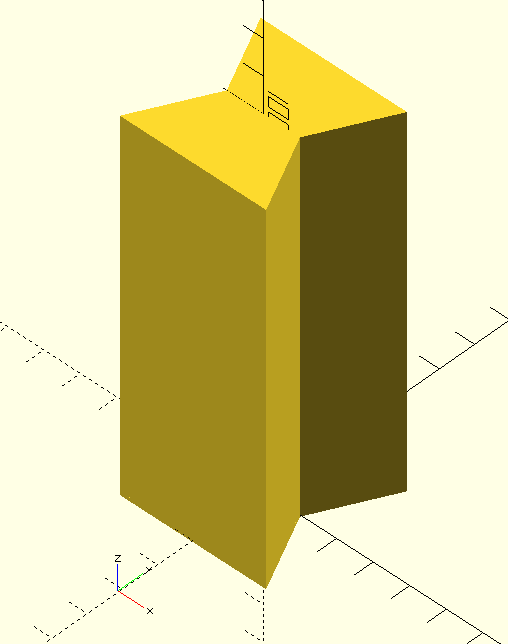
\includegraphics[width=.75\textwidth]{imagenes/extrusion-1}
    \end{minipage}
  \caption{\lstinline!polygon! extrudido mediante la operación
    \lstinline!linear_extrude!.}
  \label{fig:extrusion-1}
  \end{figure}

  
  \guillemotright El primer parámetro de \lstinline!linear_extrude!
  indica la distancia que la figura debe ser
  extrudida\footnote{Confieso que la conjugación del verbo extrudir me
    toma por sorpresa: decidí confiar en los servicios de la página
    \url{https://dle.rae.es/extrudir}.} a lo largo del eje \coord{Z}
  ---aclaró Antonia.

\subsection{\texttt{twist}}

\guillemotright Hay más posibilidades ---Antonia pareció
en\-tu\-sias\-mar\-se---: con el parámetro \lstinline!twist! podés
hacer girar la figura mientras la extrudís.


  \begin{figure}[ht]
  \begin{minipage}[]{.6\textwidth}%\vspace{0pt}
    \begin{lstlisting}
puntos = [[-20,-20],
         [-10,0],
         [-20,20],
         [20,20],
         [10,0],
         [20,-20]];

linear_extrude(100, twist=90)
  polygon(puntos);
    \end{lstlisting}
  \end{minipage}\hfill
  \begin{minipage}[]{.4\textwidth}%\vspace{0pt}
      \centering
  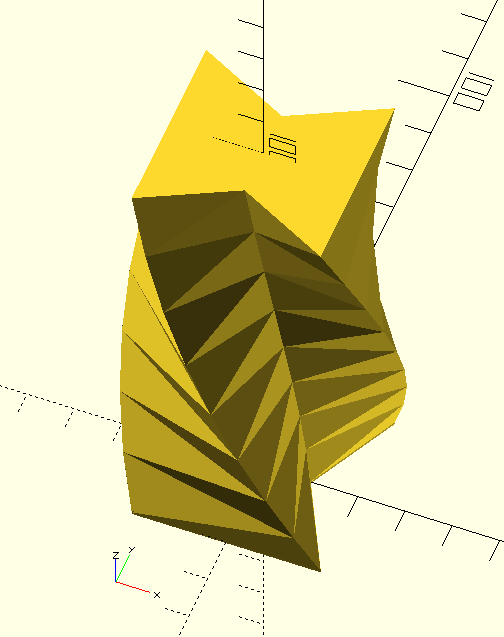
\includegraphics[width=1\textwidth]{imagenes/extrusion-twist}
    \end{minipage}
  \caption{\lstinline!polygon! extrudido y girado gracias a la opción
    \lstinline!twist! de \lstinline!linear_extrude!.}
  \label{fig:extrusion-twist}
  \end{figure}

  
  \guillemotright El valor asignado a \lstinline!twist! representa el
  giro total a lo largo de la extrusión. En el ejemplo que escribí, el
  polígono giró 90$^{\circ}$ entre las posiciones inicial y final.


 \subsection{\texttt{slices}}


 Antonia miraba el resultado con cierta insatisfacción:

 ---Por defecto, \openscad{} genera 20 `rodajas' cuando gira una
 figura durante una extrusión; por eso esa torre helicoidal nos quedó
 medio... tosca. Pero podemos hacerla más suave (o sea, con más
 `rebanadas') aprovechando el parámetro \lstinline!slices!.

  \begin{figure}[ht]
  \begin{minipage}[]{.6\textwidth}%\vspace{0pt}
    \begin{lstlisting}
puntos = [[-20,-20],
         [-10,0],
         [-20,20],
         [20,20],
         [10,0],
         [20,-20]];

linear_extrude(100, twist=90, slices=200)
  polygon(puntos);
    \end{lstlisting}
  \end{minipage}\hfill
  \begin{minipage}[]{.4\textwidth}%\vspace{0pt}
      \centering
    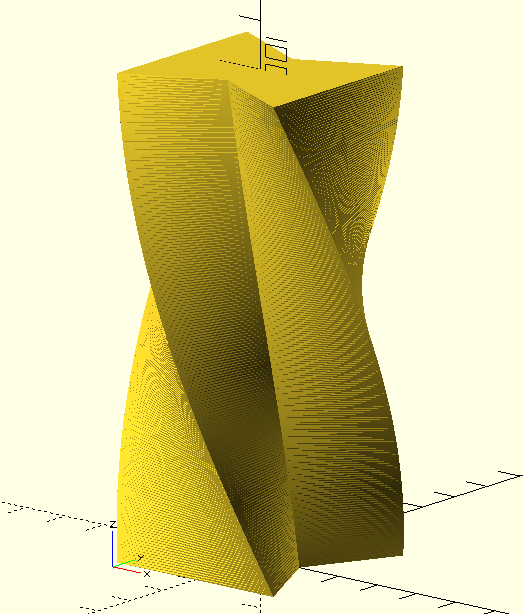
\includegraphics[width=.95\textwidth]{imagenes/extrusion-slices}
    \end{minipage}
    \caption{El \lstinline!polygon! resulta con un contorno más suave
      gracias a la opción \lstinline!slices! de
      \lstinline!linear_extrude!.}
  \label{fig:extrusion-slices}
  \end{figure}

  \guillemotright Quizá se me fue la mano con el valor 200 ---Antonia
  rio ligeramente contemplando la figura
  \ref{fig:extrusion-slices}---; pero la idea es ésa.

\subsection{\texttt{scale}}

\guillemotright Hay más, pero te molesto con la última ---rogó Antonia:

  \begin{figure}[ht]
  \begin{minipage}[]{.6\textwidth}%\vspace{0pt}
    \begin{lstlisting}
puntos = [[-20,-20],
         [-10,0],
         [-20,20],
         [20,20],
         [10,0],
         [20,-20]];

linear_extrude(100, twist=90, slices=200, scale=0)
  polygon(puntos);
    \end{lstlisting}
  \end{minipage}\hfill
  \begin{minipage}[]{.4\textwidth}%\vspace{0pt}
      \centering
    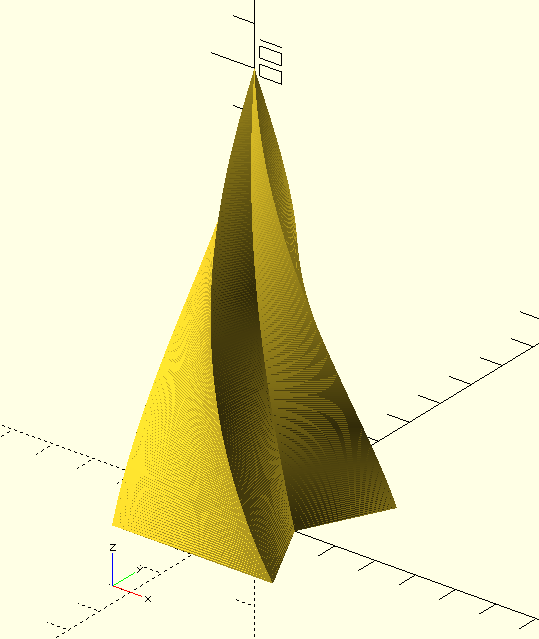
\includegraphics[width=\textwidth]{imagenes/extrusion-scale-0}
    \end{minipage}
    \caption{El \lstinline!polygon! termina su extrusión en punta
      debido al uso de la opción \texttt{scale=0} de
      \lstinline!linear_extrude!.}
  \label{fig:extrusion-scale-0}
  \end{figure}


  \guillemotright Con el parámetro \texttt{scale} podés determinar el
  tamaño de la figura en su posición final con respecto a la inicial.


  \guillemotright Con \texttt{scale=0} la figura final se anula, por
  lo que la extrusión termina en punta ---explicó Antonia, señalando
  la figura \ref{fig:extrusion-scale-0}---.  También podés, por
  supuesto, hacer que la tapa sea más grande que la base, como podés
  apreciar en la figura \ref{fig:extrusion-scale-3}.


      \begin{figure}[h!]
  \begin{minipage}[]{.6\textwidth}%\vspace{0pt}
    \begin{lstlisting}
puntos = [[-20,-20],
         [-10,0],
         [-20,20],
         [20,20],
         [10,0],
         [20,-20]];

linear_extrude(100, twist=90, slices=200, scale=3)
  polygon(puntos);
    \end{lstlisting}
  \end{minipage}\hfill
  \begin{minipage}[]{.4\textwidth}%\vspace{0pt}
      \flushright
      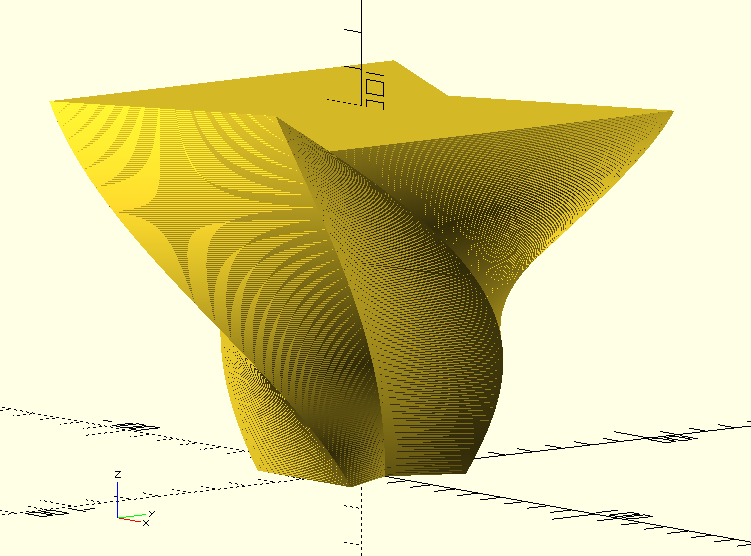
\includegraphics[width=1\textwidth]{imagenes/extrusion-scale-3}
    \end{minipage}
    \caption{\lstinline!linear_extrude! con la opción \texttt{scale=3}.}
    \label{fig:extrusion-scale-3}
  \end{figure}

  Cecilia estaba fascinada con las posibilidades, pero aún no podía
  ver qué relación mantenían con el reloj solar ansiado.

\section{Extrusión rotatoria}

---Hay una extrusión más que te quiero mostrar ---An\-to\-nia estaba
visiblemente entusiasmada---. No la vamos a usar en el reloj pero,
¿qué más da? Está muy buena.

  \begin{figure}[ht]
  \begin{minipage}[]{.55\textwidth}%\vspace{0pt}
    \begin{lstlisting}
$fn=200;

rotate_extrude(angle=360)
  translate([100,0,0])
    polygon(puntos);
    \end{lstlisting}%$
  \end{minipage}\hfill
  \begin{minipage}[]{.45\textwidth}%\vspace{0pt}
      \flushright
      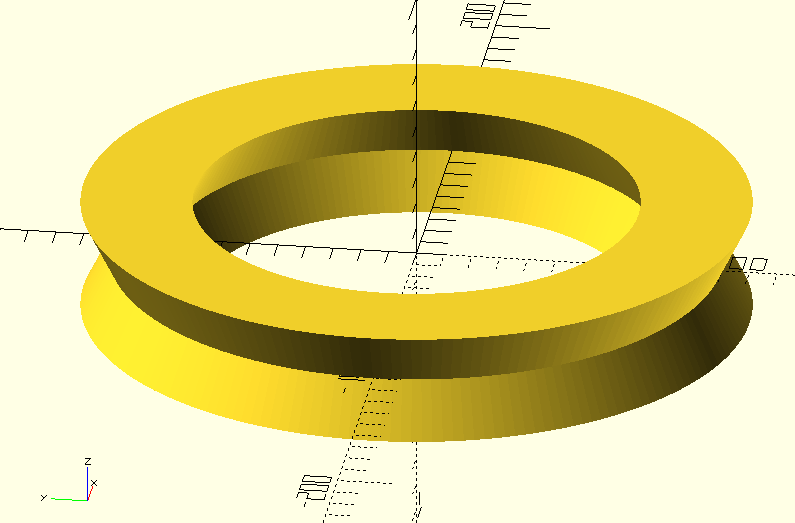
\includegraphics[width=\textwidth]{imagenes/extrusion-rotativa-1}
    \end{minipage}
    \caption{Antonia ofrece un ejemplo de \lstinline!rotate_extrude!.}
    \label{fig:extrusion-rotativa-1}
  \end{figure}


  Antonia pareció buscar la mejor manera de explicar el nuevo giro
  lingüístico:

  ---\lstinline!rotate_extrude! genera un sólido rotando alrededor del
  eje \coord{Z} un polígono cualquiera; en el ejemplo de la figura
  \ref{fig:extrusion-rotativa-1}, usé el que ya definimos antes. Es
  importante que el polígono íntegro se ubique de un mismo lado del
  eje \coord{Y} ---advirtió---; por esa razón, tuve que trasladarlo
  primero. En caso contrario, \openscad{} se hubiera quejado con un
  mensaje de error.

  Cecilia no entendía un detalle:

  ---Antonia, el polígono lo creamos recostado sobre el plano
  \coord{XY}; ¿por qué entonces aparece rotado en posición `vertical'?

  Antonia chasqueó los labios antes de contestar:

  ---Bien observado. Mirá, fue una decisión que tomaron los
  desarrolladores de \openscad{}. Supongo que les habrá parecido más
  natural que la rotación ocurriera alrededor del canónico eje
  \coord{Z}. Pero sinceramente no lo sé; el hecho es que es así ---la
  última frase fue pronunciada por Antonia con tono de no admitir
  réplica. Cecilia, por su parte, tampoco encontró necesario
  discutirla.

  \guillemotright Si nuestra intención es obtener algo así como
  nuestro polígono rotado alrededor del eje \coord{Z}, debemos crear
  otro que sea su estricta mitad en las \coord{Y} positivas (o
  negativas) ---dijo Antonia, ahora con tono negociador.

  
  \begin{figure}[ht]
  \begin{minipage}[]{.5\textwidth}%\vspace{0pt}
    \begin{lstlisting}
puntos2 = [[0,-20],
          [0,20],
          [20,20],
          [10,0],
          [20,-20]];
          
polygon(puntos2);
    \end{lstlisting}
  \end{minipage}\hfill
  \begin{minipage}[]{.5\textwidth}%\vspace{0pt}
    \flushright
      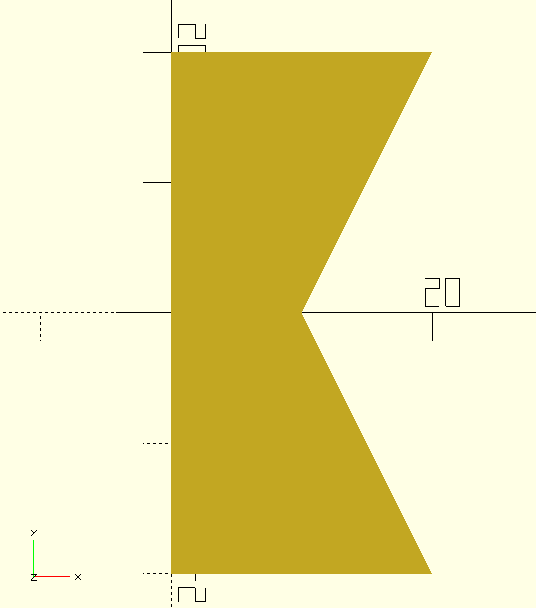
\includegraphics[width=.5\textwidth]{imagenes/poligono-2}
    \end{minipage}
    \caption{Antonia crea un nuevo polígono...}
    \label{fig:poligono-2}
  \end{figure}


  \begin{figure}[ht]
  \begin{minipage}[]{.5\textwidth}%\vspace{0pt}
\begin{lstlisting}
$fn=200;

rotate_extrude(angle=360)
   polygon(puntos2);
    \end{lstlisting}%$
  \end{minipage}\hfill
  \begin{minipage}[]{.5\textwidth}%\vspace{0pt}
      \flushright
      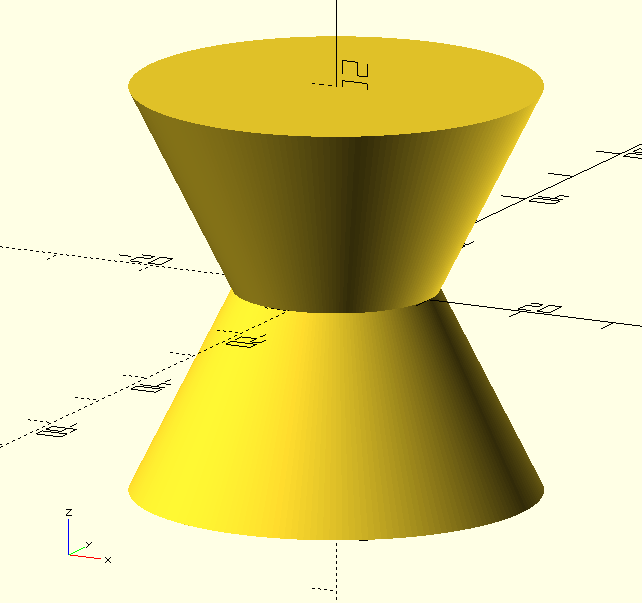
\includegraphics[width=.8\textwidth]{imagenes/rotate-extrude-2}
    \end{minipage}
    \caption{...para que \lstinline!rotate_extrude! cree con él un
      cuerpo que resulte una suerte de versión con simetría radial del
      polígono con el que comenzó el presente capítulo.}
    \label{fig:rotate-extrude-2}
  \end{figure}


  \guillemotright Como sin duda ya habrás sospechado, el ángulo puede
  ser cualquiera ---agregó Antonia, señalando la figura
  \ref{fig:rotate-extrude-3}.

  \begin{figure}[ht]
  \begin{minipage}[]{.5\textwidth}%\vspace{0pt}
\begin{lstlisting}
$fn=200;
rotate_extrude(angle=150)
  translate([100,0,0])
    polygon(puntos);
  
rotate_extrude(angle=250)
   polygon(puntos2);
    \end{lstlisting}%$
  \end{minipage}\hfill
  \begin{minipage}[]{.5\textwidth}%\vspace{0pt}
      \flushright
      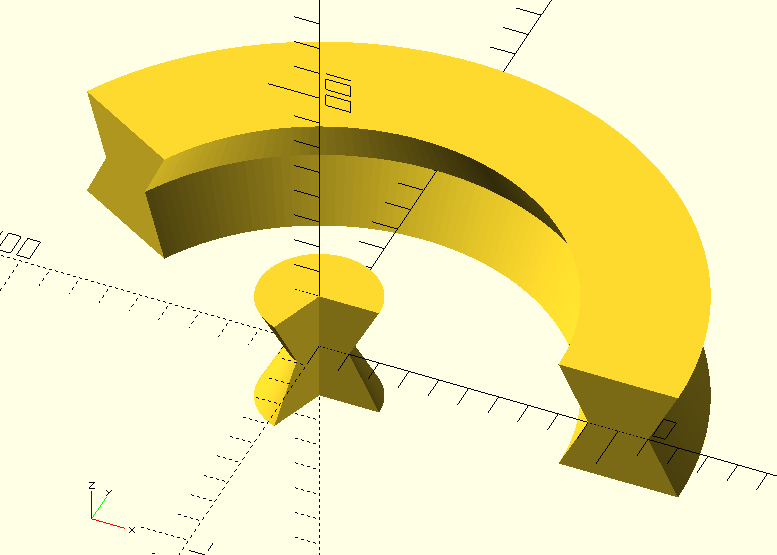
\includegraphics[width=.9\textwidth]{imagenes/rotate-extrude-3}
    \end{minipage}
    \caption{El ángulo usado por \lstinline!rotate_extrude! no tiene
      porqué ser igual 360$^{\circ}$.}
    \label{fig:rotate-extrude-3}
  \end{figure}


  \section{Dos figuras especiales}

  \guillemotright Dos más y terminamos por hoy ---aseguró Antonia---.
  Hay dos figuras especiales que seguramente querrás conocer: con
  \lstinline!circle(r=radio)! creás un círculo, y con
  \lstinline!square([ancho, alto], center)!  creás... bueno, creo que
  no hace falta que te lo diga.

  
  \begin{figure}[ht]
  \begin{minipage}[]{.5\textwidth}%\vspace{0pt}
    \begin{lstlisting}
rotate_extrude(angle=360)
  translate([70,0,0])
    circle(r=10);
  \end{lstlisting}
%   \end{center}
%   \begin{center}
\end{minipage}\hfill
\begin{minipage}[]{.5\textwidth}%\vspace{0pt}
  \flushright
  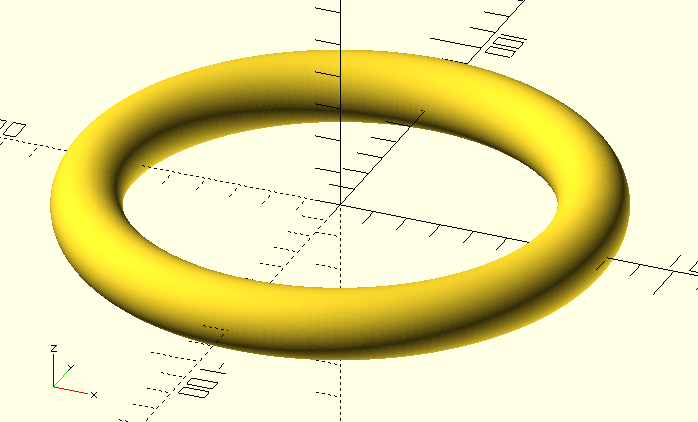
\includegraphics[width=.9\textwidth]{imagenes/rotate-circle}
\end{minipage}
\caption{Antonia somete un \lstinline!circle! a la transformación
  \lstinline!rotate_extrude!.}
    \label{fig:rotate-circle}
  \end{figure}%
  \begin{figure}[h!]
  \begin{minipage}[]{.5\textwidth}%\vspace{0pt}
    \begin{lstlisting}
rotate_extrude(angle=360)
  translate([70,0,0])
    square([10,30], center=true);
  \end{lstlisting}
  % \end{center}
  % \begin{center}
\end{minipage}\hfill
\begin{minipage}[]{.5\textwidth}%\vspace{0pt}
  \flushright
  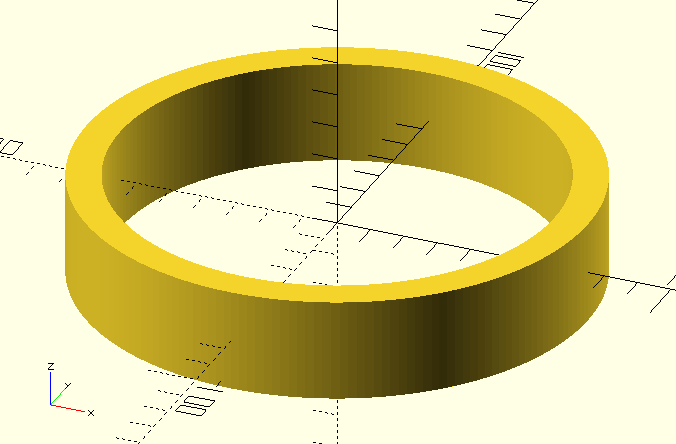
\includegraphics[width=.9\textwidth]{imagenes/rotate-square}
\end{minipage}
\caption{Antonia aplica la transformación \lstinline!rotate_extrude! a
  un \lstinline!square!.}%\iftoggle{libro}{\vspace{128in}}{}
    \label{fig:rotate-square}
  \end{figure}

  
  
   Cecilia, a esta altura del capítulo, realmente ya no necesitaba que
   le dijera nada: sólo quería descansar.




%%% Local Variables:
%%% mode: latex
%%% TeX-master: "../libro"
%%% End:

